\documentclass[paper=a4, fontsize=11pt]{article} % A4 paper and 11pt font size
%\usepackage[utf8x]{inputenc}
%\usepackage[czech]{babel} % English language/hyphenation
\usepackage{amsmath,amsfonts,amsthm} % Math packages
%\usepackage{lipsum} % Used for inserting dummy 'Lorem ipsum' text into the template
%\usepackage{sectsty} % Allows customizing section commands
%\allsectionsfont{\centering \normalfont\scshape} % Make all sections centered, the default font and small caps
\usepackage{fancyhdr} % Custom headers and footers
\pagestyle{fancyplain} % Makes all pages in the document conform to the custom headers and footers
\fancyhead{} % No page header - if you want one, create it in the same way as the footers below
\fancyfoot[L]{} % Empty left footer
\fancyfoot[C]{\thepage} % Empty center footer
\fancyfoot[R]{} % Page numbering for right footer
\renewcommand{\headrulewidth}{0pt} % Remove header underlines
\renewcommand{\footrulewidth}{0pt} % Remove footer underlines
\usepackage{graphicx}
\usepackage{indentfirst}
\usepackage[table]{xcolor}
\usepackage{booktabs}
\newcommand{\ra}[1]{\renewcommand{\arraystretch}{#1}}
\setlength\parindent{20pt} % Removes all indentation from paragraphs - comment this line for an assignment with lots of text
\usepackage{amssymb}
% Margins
\topmargin=-0.45in
\evensidemargin=0.0in
\oddsidemargin=-0.5in
\hoffset=1.0in
\textwidth=5.5in
\textheight=9.0in
\headsep=0.25in
%----------------------------------------------------------------------------------------
%	TITLE SECTION
%----------------------------------------------------------------------------------------

\newcommand{\horrule}[1]{\rule{\linewidth}{#1}} % Create horizontal rule command with 1 argument of height

\title{	
\normalfont \normalsize 
\textsc{Norwegian University of Science and Technology} \\ [25pt] % Your university, school and/or department name(s)
\horrule{0.5pt} \\[0.4cm] % Thin top horizontal rule
\huge Using Minimax with Alpha-Beta pruning to play Quarto\\ % The assignment title
\horrule{2pt} \\[0.5cm] % Thick bottom horizontal rule
}

\author{Jan Bednarik\\Tomas Dohnalek} % Your name

\date{\normalsize\today} % Today's date or a custom date

\begin{document}

\maketitle % Print the title

\section{Introduction}


The game called Quarto is a puzzle game that somewhat resembles of the well known game Tic-tac-toe. As far as the artificial intelligence of computer driven player is concerned the game seems to be way more complex though. The game board consists of the 16 fields and each player can choose from the 16 different pieces that are placed on board in an iterative manner. What is more each player chooses the piece for his opponent and this fact makes the game state space even more complex.

Given the computational difficulty the artificial player is not able to explore entirely all of the game states. Therefore it is necessary to come up with the right heuristic functions that would be both time efficient and would return the value that describes the game state the best.

We will first introduce our implementation and then we will explain our chosen heuristics. In the end we will present the results both from the testing within our application and from the Quarto tournament.

\section{Implementation}
This section is devoted to the technical details of our implementation. In section \ref{txt:tech} the technologies we utilized are listed, section \ref{txt:arch} gives the brief description of the overall architecture and the section \ref{txt:evalfunc} presents the state evaluation algorithm and the heuristics we designed.

\subsection{Chosen technologies} \label{txt:tech}
The core alpha-beta algorithm and the evaluation function might be computationally demanding as the evaluator needs to explore the immense state space. Therefor we decided to use the C++ programming language as the executable binary tends to run faster compared to the interpreted programs. We also use th Qt libraries because its inbuilt containers and network programming support simplifies the implementation.

\subsection{Architecture} \label{txt:arch}

The game is run as a console application and the types of the players can be set using the program parameters.

\subsection{State evaluation function} \label{txt:evalfunc}

There are two main requirements that the good state evaluation function must fulfil - it should both return the values that comply with the player's intention to win and it should be time efficient. The first possible naive approach is to examine whether the opponent might win in the next move and the second more complex approach is to examine the number of the pieces the player can choose from so that he would not loose.

\subsubsection{Heuristic 1 - The victory}

This is the easiest heuristic each beginner player can think of. In every move we just check whether the piece the player chooses would not enable the opponent to win in the next move. Using this heuristic the minimax player of the level 1 is somewhat similar to the novice player. However the minimax player of the greater level can beat the novice player as the minimax can estimate the path to the victory better.

\subsubsection{Heuristic 2 - Odd or even}

how many triplets\footnote{(By triplet we refer to the the three pieces that have at least one common property and that are placed either in the same row, column or diagonal.} are currently placed on the game board.

Let's say there is just one triplet with the pieces sharing just one common property present on the game board. Given the fact both players intend to win they will be choosing the pieces of the opposite property (as compared to the triplet's property) in their next moves. The player who chooses the piece for his opponent can therefore easily see whether the situation is good or bad for him by the number of remaining pieces of the opposite property. If the number is even this player will potentially loose in the next moves as he might be sooner or later forced to give his opponent the piece of the property that the pieces in triplet share.

The figure \ref{fig:1triplet} shows the situation when exactly one triplet is placed on the board. It can be noticed that the three pieces contained in the only triplet share one common property - they are all big. The player who chooses the piece should only pick the small piece for his opponent. We can see there are 7 small pieces to choose from and as this is an odd number the situation for this player looks promising.

\begin{figure}[!htb]
	\centering
		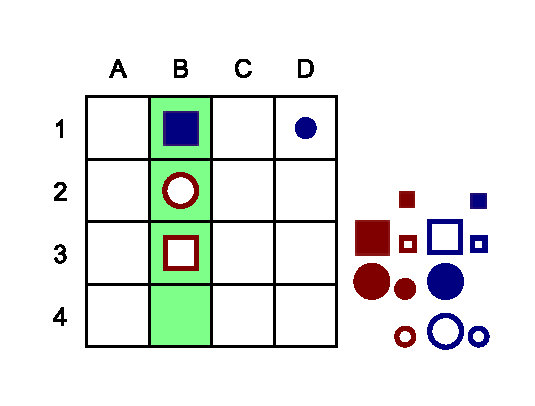
\includegraphics[width=10cm]{img/eval_func_1triplet.eps}
	\caption{1 triplet}
	\label{fig:1triplet}
\end{figure}

Sadly the situation might (and will) get more complicated when more pieces are placed on board. The figure \ref{fig:2triplets} shows the situation when two different triplets are present on the board. The pieces of the vertical triplet are all big and the pieces of the horizontal triplet are all blue. The player who chooses the piece for his opponent should now pick the small piece and also the red piece. If we examine the remaining pieces we can notice there are seven small pieces and 6 red pieces remaining - an odd and an even number. The situation is now both good and bad for the player.

\begin{figure}[!htb]
	\centering
		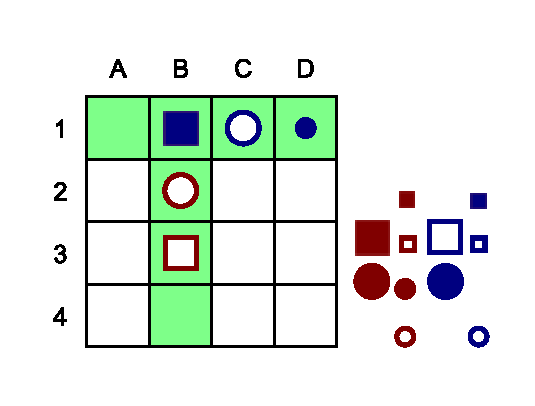
\includegraphics[width=10cm]{img/eval_func_2triplets.eps}
	\caption{2 triplets}
	\label{fig:2triplets}
\end{figure}

Given this inconsistency we had to adjust our final approach. For each game state we examine the board and count the pieces that the player can choose for his opponent so that he would not loose in the next move. Example situation can be seen on the figure \ref{fig:even} where the \textit{good} and \textit{bad} pieces are listed. It is obvious that the player can choose only two pieces and as this is the even number we evaluate this game state as inconvenient for the player.


\begin{figure}[!htb]
	\centering
		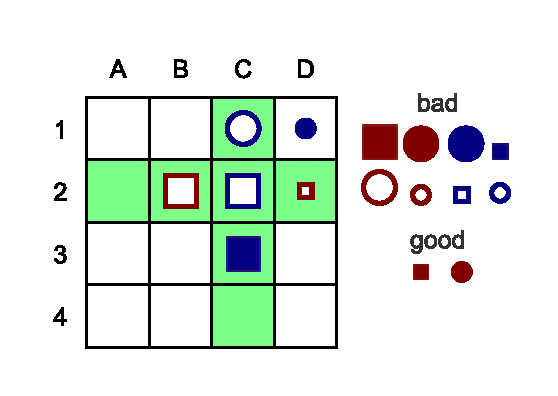
\includegraphics[width=10cm]{img/eval_func_even.eps}
	\caption{Even number of remaining pieces.}
	\label{fig:even}
\end{figure}

We also estimate how good or bad this situation is for the player by the number of the pieces he can choose from. The higher this number is the less significant this position is as the game state can change easily in the next moves. However if the number is low (let's say just 2) the game state will hardly change in the next moves.

In the greater detail we just subtract the number of these pieces from the positive infinity (represented by number 1024) in case an odd number of "good" pieces are remaining or we add this number to the negative infinity (represented by number -1024) in case of the even number of "good" pieces are remaining.








\section{Results}

In this section we present results of some matches between our-implemented players and also results of our special player Minimax-0 in tournament.

\subsection{Random versus Novice}
You can see the results if 100 games in figure \ref{fig:random-novice}. 
In half of the games started Random, in the other half it was Novice.



\begin{figure}[ht]
    \begin{minipage}[c]{0.40\linewidth}
        \centering
        \ra{1.3}
        \begin{tabular}{cll}
            \toprule
            \textcolor{red!100}{$\bullet$} & Random wins & 3       \\
            \textcolor{blue!100!yellow!100!red!80}{$\bullet$} & Novice wins & 97      \\  
            \bottomrule
        \end{tabular}
    \end{minipage}
    \begin{minipage}[c]{0.60\linewidth}
        \centering
        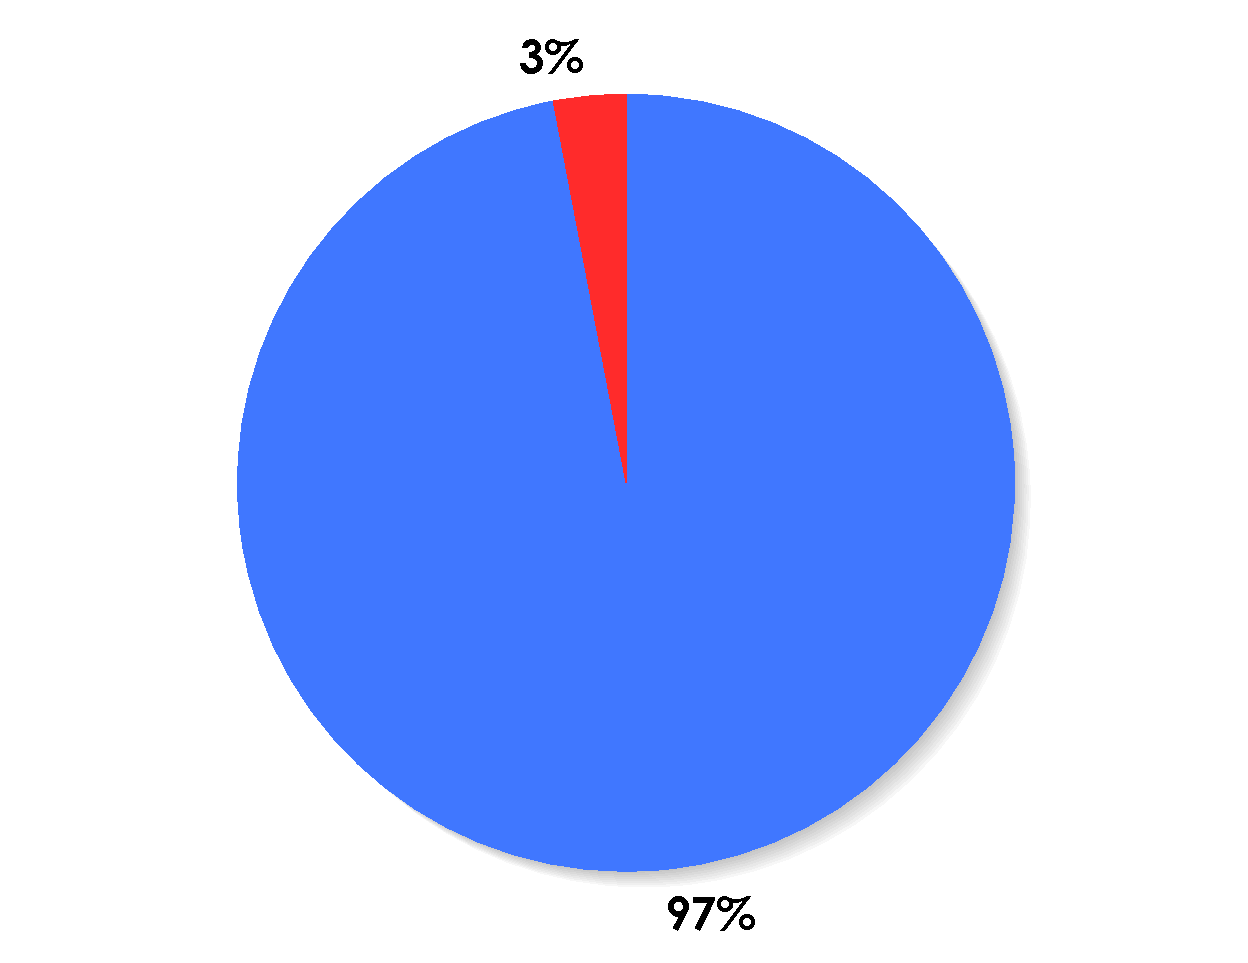
\includegraphics[scale=0.35]{img/random-novice.pdf}
    \end{minipage}
    \caption{100 games of Random against Novice.}
    \label{fig:random-novice}
\end{figure}



\subsection{Novice versus Minimax-3}
You can see the results if 20 games in figure \ref{fig:novice-minimax3}. 
In half of the games started Novice, in the other half it was Minimax-3.

\begin{figure}[ht]
    \begin{minipage}[c]{0.40\linewidth}
        \centering
        \ra{1.3}
        \begin{tabular}{cll}
            \toprule
            \textcolor{red!100}{$\bullet$} & Novice wins & 1       \\
            \textcolor{blue!100!yellow!100!red!80}{$\bullet$} & Minimax-3 wins & 18      \\  
            \textcolor{gray!100}{$\bullet$} & Draws & 1      \\  
            \bottomrule
        \end{tabular}
    \end{minipage}
    \begin{minipage}[c]{0.60\linewidth}
        \centering
        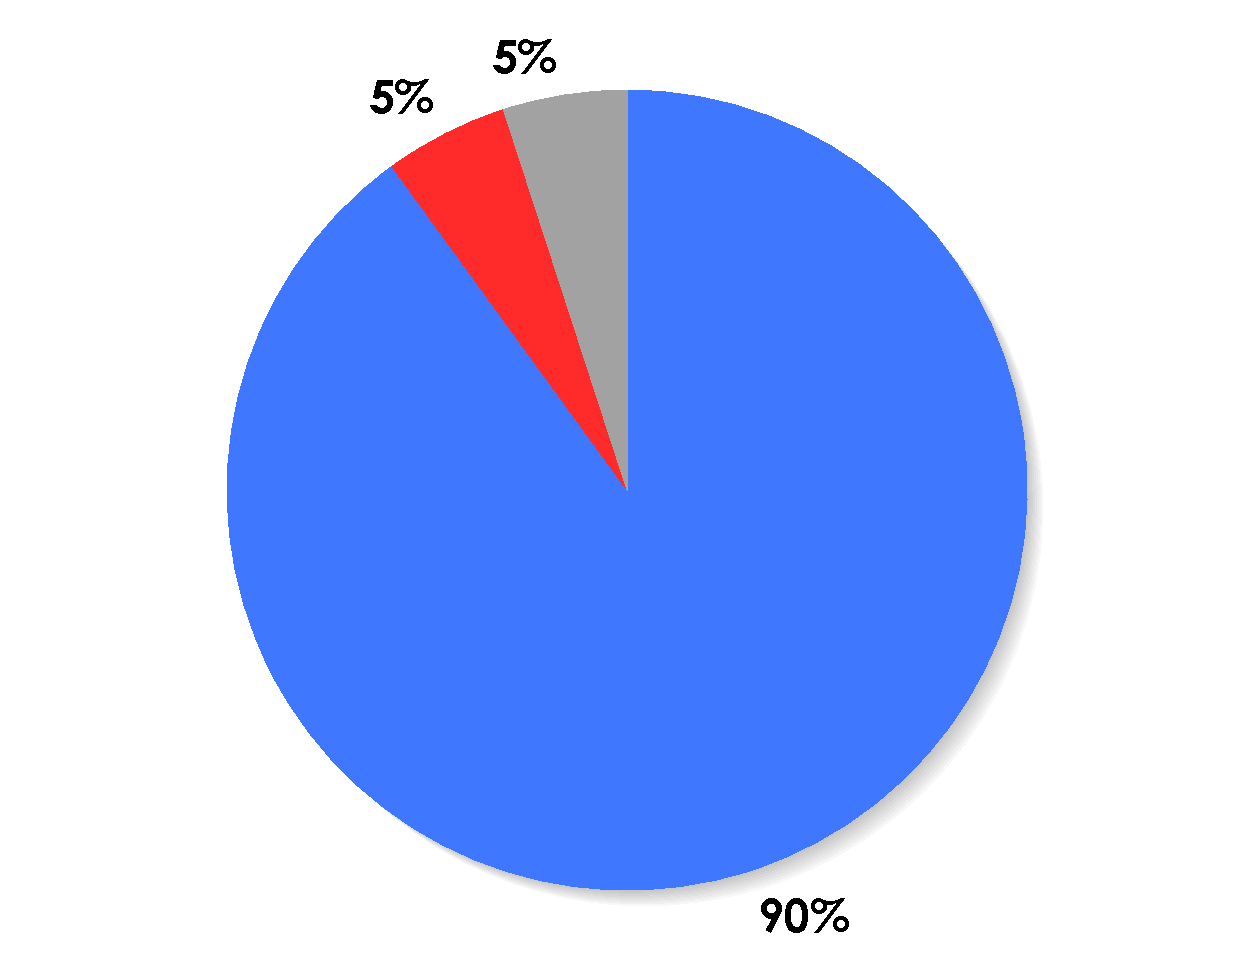
\includegraphics[scale=0.35]{img/novice-minimax3.pdf}
    \end{minipage}
    \caption{20 games of Novice against  Minimax-3.}
    \label{fig:novice-minimax3}
\end{figure}


\subsection{Minimax-3 versus Minimax-4}
You can see the results if 20 games in figure \ref{fig:minimax3-minimax4}. 
In half of the games started Minimax-3, in the other half it was Minimax-4.


\begin{figure}[ht]
    \begin{minipage}[c]{0.40\linewidth}
        \centering
        \ra{1.3}
        \begin{tabular}{cll}
            \toprule
            \textcolor{red!100}{$\bullet$} & Minimax-3 wins & 2       \\
            \textcolor{blue!100!yellow!100!red!80}{$\bullet$} & Minimax-4 wins & 9      \\  
            \textcolor{gray!100}{$\bullet$} & Draws & 9      \\  
            \bottomrule
        \end{tabular}
    \end{minipage}
    \begin{minipage}[c]{0.60\linewidth}
        \centering
        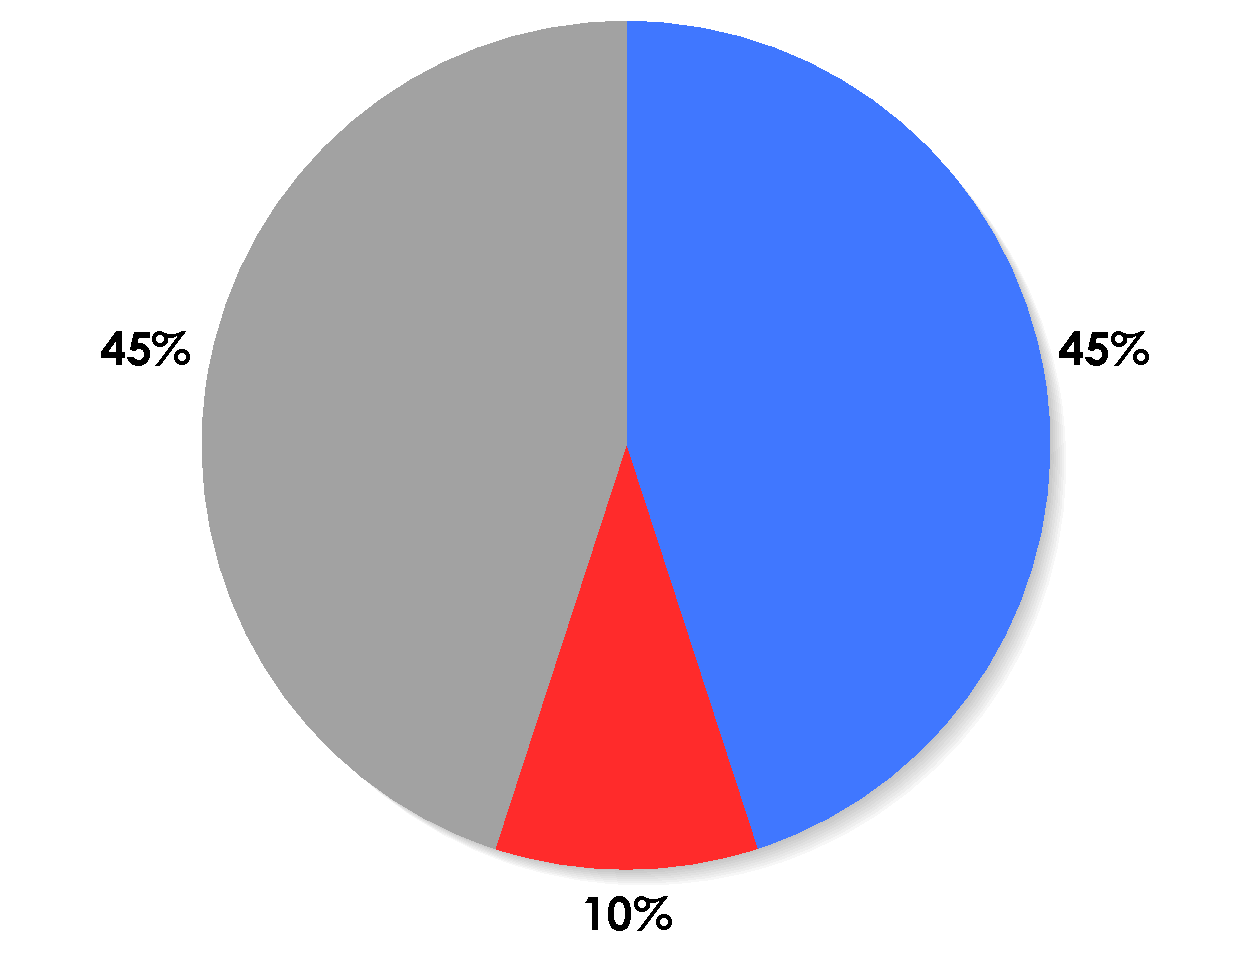
\includegraphics[scale=0.35]{img/minimax3-minimax4.pdf}
    \end{minipage}
    \caption{20 games of Minimax-3 against Minimax-4.}
    \label{fig:minimax3-minimax4}
\end{figure}

\subsection{Minimax in tournament}
We have played 20 games with our Minimax-4 player against Dominik's and Pablo's player.
Results can be seen in figure \ref{fig:tournament}.
In half of the games started our player, in the other half it was player of Dominik and Pablo.

\begin{figure}[ht]
    \begin{minipage}[c]{0.40\linewidth}
        \centering
        \ra{1.3}
        \begin{tabular}{cll}
            \toprule
            \textcolor{red!100}{$\bullet$} & Dominik's and Pablo's wins & 0       \\
            \textcolor{blue!100!yellow!100!red!80}{$\bullet$} & Our Minimax-4  wins & 18      \\  
            \textcolor{gray!100}{$\bullet$} & Draws & 2      \\  
            \bottomrule
        \end{tabular}
    \end{minipage}
    \begin{minipage}[c]{0.60\linewidth}
        \centering
        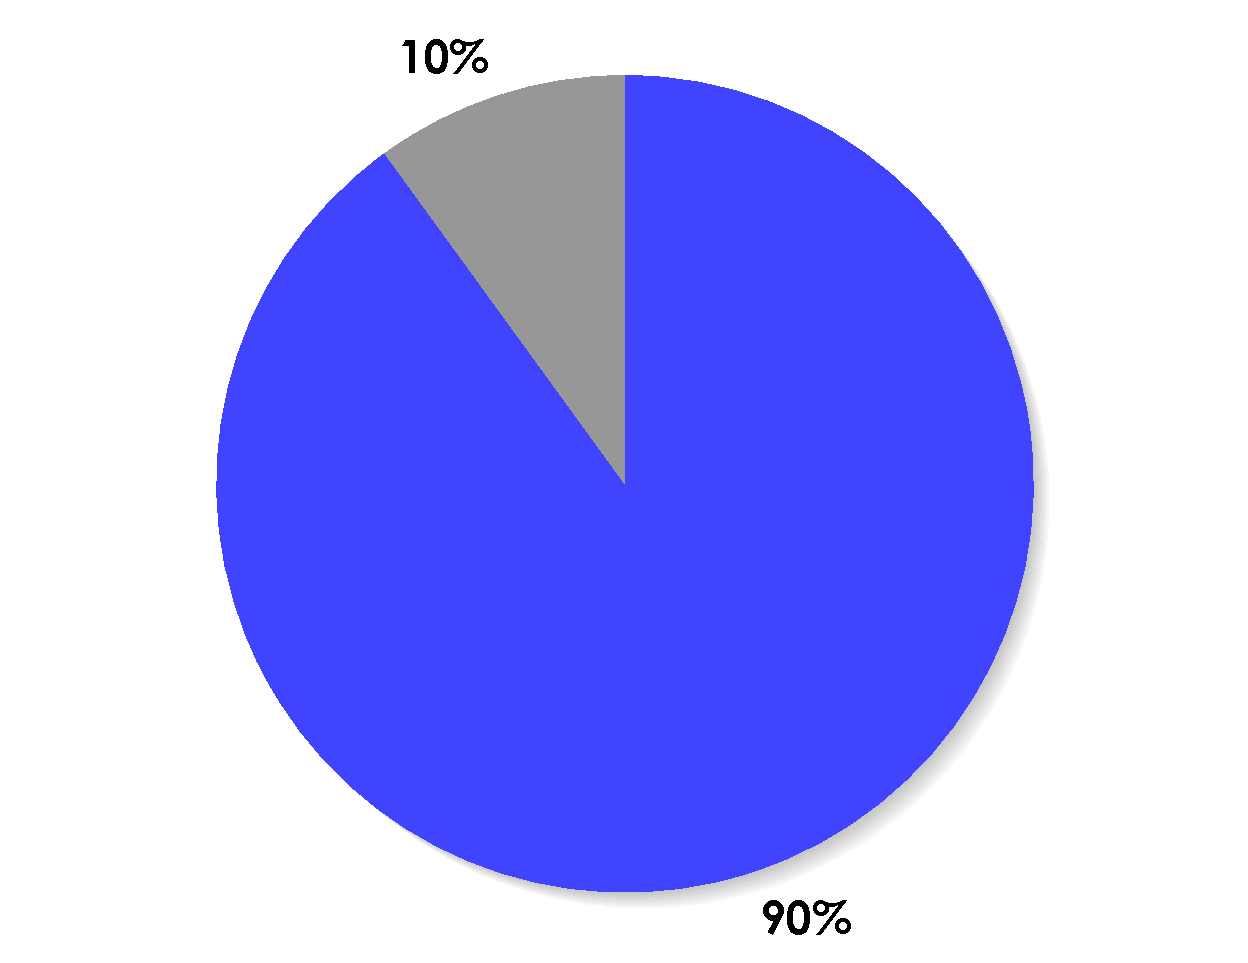
\includegraphics[scale=0.35]{img/tournament.pdf}
    \end{minipage}
    \caption{20 games of Dominik's and Pablo's Minimax-4 against our Minimax-4.}
    \label{fig:tournament}
\end{figure}


We have also played 20 games with our Minimax-4 player against Marc's and Valerio's player.
Results can be seen in figure \ref{fig:tournament2}.
\begin{figure}[ht]
    \begin{minipage}[c]{0.40\linewidth}
        \centering
        \ra{1.3}
        \begin{tabular}{cll}
            \toprule
            \textcolor{red!100}{$\bullet$} & Marc's and Valerio's wins & 0       \\
            \textcolor{blue!100!yellow!100!red!80}{$\bullet$} & Our Minimax-4  wins & 20      \\  
            \textcolor{gray!100}{$\bullet$} & Draws & 0      \\  
            \bottomrule
        \end{tabular}
    \end{minipage}
    \begin{minipage}[c]{0.60\linewidth}
        \centering
        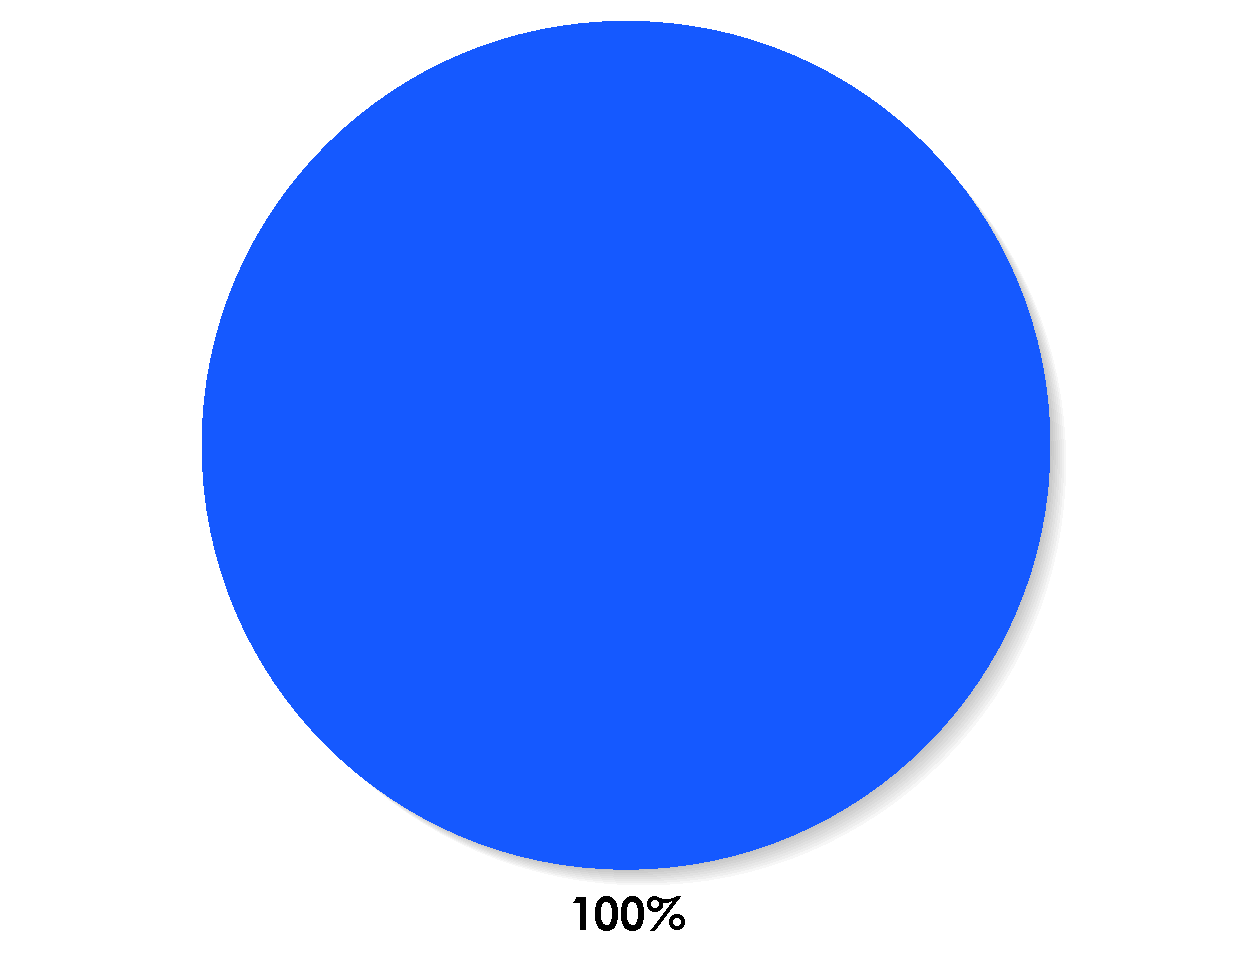
\includegraphics[scale=0.35]{img/tournament2.pdf}
    \end{minipage}
    \caption{20 games of Marc's and Valerio's Minimax-4 against our Minimax-4.}
	\label{fig:tournament2}
\end{figure}


%%%
Unfortunately we could not play against Marc's and Valerio's player because they were not able to implement network module for this project in time.
%%


\section{Reflection}
In this section we will reflect our experience with programming for the tournament and also the participation in tournament itself.

\subsection{Experience of programming for tournament}
During designing architecture of our program, we had a short  meeting with other teams and we have decided to use client-server architecture. 
We did not design any protocol at that moment.

As Dominik and Pablo have finished their implementation early, they suggested that they can create simple server as an extension to their application. 
They have made their own protocol and implemented the server and example of client in Java. 
As we use C++/Qt we did not have to implement client from scratch, we could use some Qt classes that let us work over network very easily. 

The biggest issue was connected with fact that our architecture was not designed to play repeated games (as we intended to run repeated games in simple loop from shell) and we had to redesign and reimplement some parts of our code. We have also encountered issues related to networking and understanding the protocol.

\subsection{Participation in tournament}
We have created special player called \emph{Minimax-0} which had no fixed depth of alphabeta search and use variable depth instead. As game continues we increase the depth because the search space is getting rapidly smaller after each turn. From 8th move we were able to use Minimax-8 and so we could explore the search space entirely. In the beginning of tournament we have agreed with our opponents that we would not player and use Minimax-4 instead.


%Our client has won most of the games and we were of course satisfied with this result. After the tournament we have discussed our strategy with our opponents and we have figured out that the main difference is of course in evaluation function. Ours was probably much more powerful. It was really helpful to have a opportunity to compare our state-evaluated function against other teams.	

As Marc and Valerio were not able to finish they program, we played only against Dominik's and Pablo's player. Our client has won most of the games and we were of couse satisfied with this results. After the tournament we have discussed our strategy with our opponents and we figured out that the main difference is of course in evaluation function. Ours was probably much more powerful.

\section{Summary}
Goal of this project was to create a working program playing game called Quarto.
We have implemented several different kinds of players such as Random, Novice, Minimax with different depths of search, Human player and also Remote player who can be some other application. 
%%
We have participated in tournament with two other teams; unfortunately one team was not able to deliver their application so we had to play only against once client. 
%%
Implemented Minimax player was able to easily beat all other opponents including some applications we have explored on the Internet. 
It would be nice to compare our Minimax player with even more applications so we can learn if used state-evaluation method was powerful enough.

%-----------------------------------------------
\begin{flushleft}
%\bibliography{literatura} % viz. literatura.bib..
%\bibliographystyle{czplain}
\end{flushleft}
\end{document}
